\documentclass{article}

% Language setting
% Replace `english' with e.g. `spanish' to change the document language
\usepackage[english]{babel}

% Set page size and margins
% Replace `letterpaper' with `a4paper' for UK/EU standard size
\usepackage[letterpaper,top=2cm,bottom=2cm,left=3cm,right=3cm,marginparwidth=1.75cm]{geometry}

% Useful packages
\usepackage{amsmath}
\usepackage{graphicx}
\usepackage[colorlinks=true, allcolors=blue]{hyperref}
\usepackage{url}
\usepackage{appendix}

\usepackage{color}
\usepackage{listings}
\lstset{ %
language=C++,                % choose the language of the code
basicstyle=\footnotesize,       % the size of the fonts that are used for the code
numbers=left,                   % where to put the line-numbers
numberstyle=\footnotesize,      % the size of the fonts that are used for the line-numbers
stepnumber=1,                   % the step between two line-numbers. If it is 1 each line will be numbered
numbersep=5pt,                  % how far the line-numbers are from the code
backgroundcolor=\color{white},  % choose the background color. You must add \usepackage{color}
showspaces=false,               % show spaces adding particular underscores
showstringspaces=false,         % underline spaces within strings
showtabs=false,                 % show tabs within strings adding particular underscores
frame=single,           % adds a frame around the code
tabsize=2,          % sets default tabsize to 2 spaces
captionpos=b,           % sets the caption-position to bottom
breaklines=true,        % sets automatic line breaking
breakatwhitespace=false,    % sets if automatic breaks should only happen at whitespace
escapeinside={\%*}{*)}          % if you want to add a comment within your code
}



\title{COMP5048 Assignment 1A}
\author{YIYANG XU 540840166}

\begin{document}

\tableofcontents

\maketitle

\begin{abstract}
Assignment 1A of COMP5048.
\end{abstract}

\section{Category A}

\subsection{Visual Analysis 1}

\begin{figure}[h]
\centering
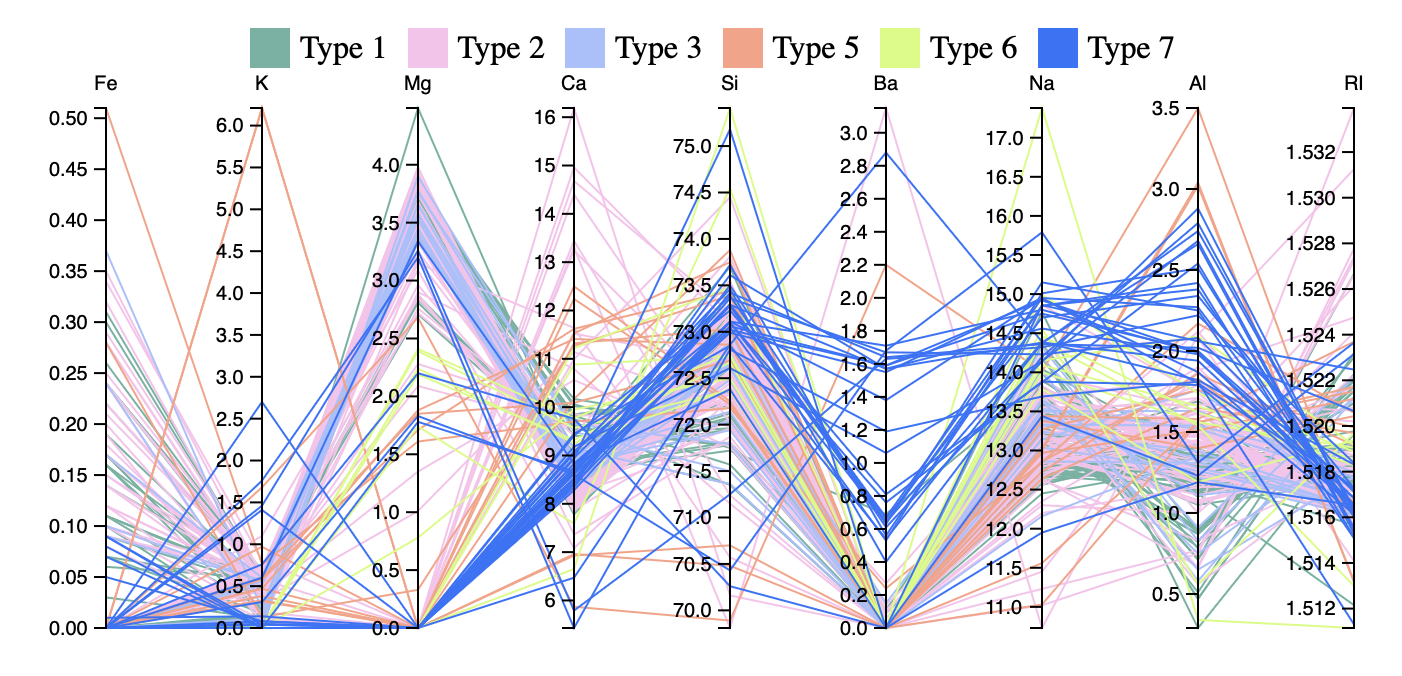
\includegraphics[width=0.8\textwidth]{Task1_1_D3.png}
\caption{Parallel coordinates use D3}
\end{figure}

\begin{figure}[h]
\centering
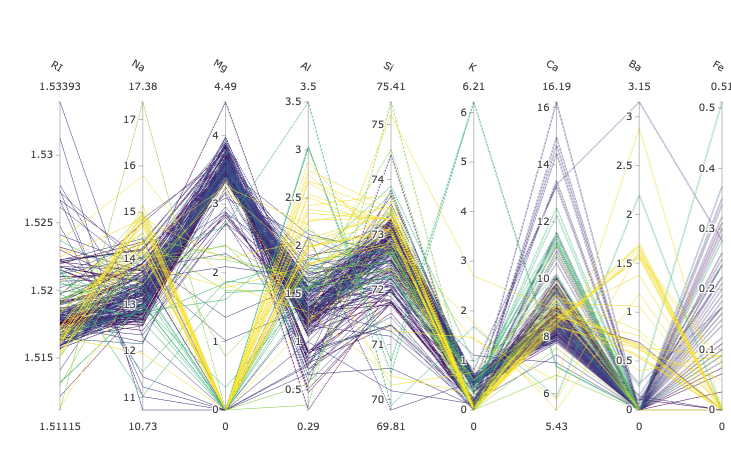
\includegraphics[width=0.7\textwidth]{Task1_1_R.png}
\caption{Parallel coordinates use R}
\end{figure}

\newpage

\subsection{Discussion on Visual Analysis 1}

\subsubsection{Design}

\indent

I use D3.js and R to generate the parallel coordinates for "glass.csv". The classification criterion on the images is the "Type" column. I hope to show the relations between the refractive index and the ingredients among different types of glass.

Change the order of columns in the D3 project, while the R project remains in the original order. I will use this D3 project to explain the correlation, similarity, and cluster of data.

\subsubsection{Evaluation}

\indent 

The main discussion of this graph is to find the relation among different ingredients due to the glass type. 

First, for correlation. Some of the ingredients data shows a strong correlation with the glass type. Taking Glass Type 7 and Type 2 as examples, Glass Type 7 contains much less Fe, K and Mg than other types. However, it contains more Ba and Al than most other types. Glass Type 2 contains much more Ca than the others. We also find that Glass Type 2 has the highest refractive index. There may be a correlation between the refractive index and the Ca content. 

We also find that the lines between Na and Al intersect, which may show that their content is negatively correlated. The line between Si and Ba has a similar tendency, which may show that their content is positively correlated.

Second, for similarity. Glass Type 2, Type 3, Type 5 and Type 6 show huge similarity in some ingredient content. They all have a closer Mg, Ca, Ba, and Na content. All of them have a similar refractive index, which may also show the relation between these ingredients and the refractive index. 

Third, for cluster. Taking Glass Type 7 as an example, Type 7 glass has the cluster in ingredient Fe, Ca, Si and Na. This shows that Type 7 glass has similar attributes due to these ingredients. In addition, we find that Type 7 has a cluster in the refractive index, which is about 1.516-1.518. We may find relations among these clusters. 

Fourth, for outline points. It will be easy to find the outline points from the parallel coordinates. For example, there exists an outline point for Glass Type 5 in Fe content (0.50), an outline point for Type 5 in K content (6.0), and an outline point for Type 5 in Al content(3.5). These outline points may show that the data in these glasses have errors, and the points may need to be cleaned or fixed before further study.

\subsubsection{Pros and Cons}

I suppose that parallel coordinates have 3 advantages and 3 disadvantages.

\bigskip

\noindent\textbf{Advantages}

1. Easy to show multi-dimensional data. As for the X-axes that can be easily spread, it can be used to show a huge amount of dimensions. If we need to add dimension, it is also easy to add new Y-axes. In this example, it is easy to remove the "Type" axis and move other axis to change their orders.

2. Easy to make sense of its structure. The parallel coordinates have a simple data structure. In this project, we can easily understand that the color means a different type, while the intersection of each line and the axis shows the data of each glass.

3. Easy to show simple relations. We can easily guess the negative or positive relations from the lines of the graph, such as guessing the negative relation between Na and Al and the positive relation between Si and Ba.

\bigskip

\noindent\textbf{Disadvantages}

1. Hard to recognize the line when processing a huge amount of data. In this project, we may find that the relation between Na and Al may be difficult to recognize its type.

2. Strongly dependent on the order of axes, may cause loss attribute. We have to choose the order of axes curiously, and these choosing process are easy to lose the relation between axes which are not closer. In this project, it may be hard to find the relation between Fe and Al from the graph.

3. Available only for numeric data. It may be difficult to show other types of data.

\newpage

\subsection{Visual Analysis 2}

\begin{figure}[h]
\centering
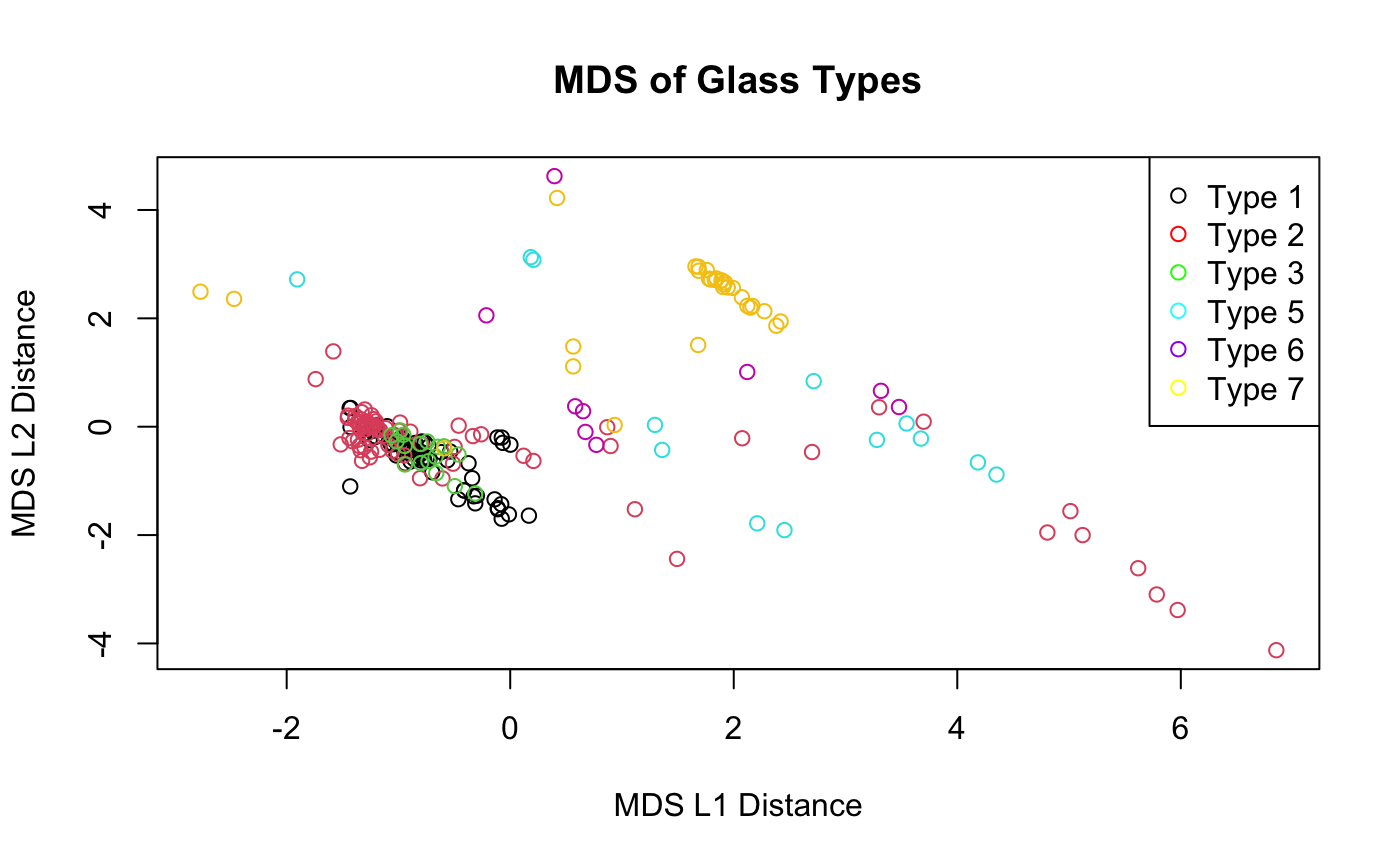
\includegraphics[width=0.7\textwidth]{MDS.png}
\caption{MDS use R}
\end{figure}

\begin{figure}[h]
\centering
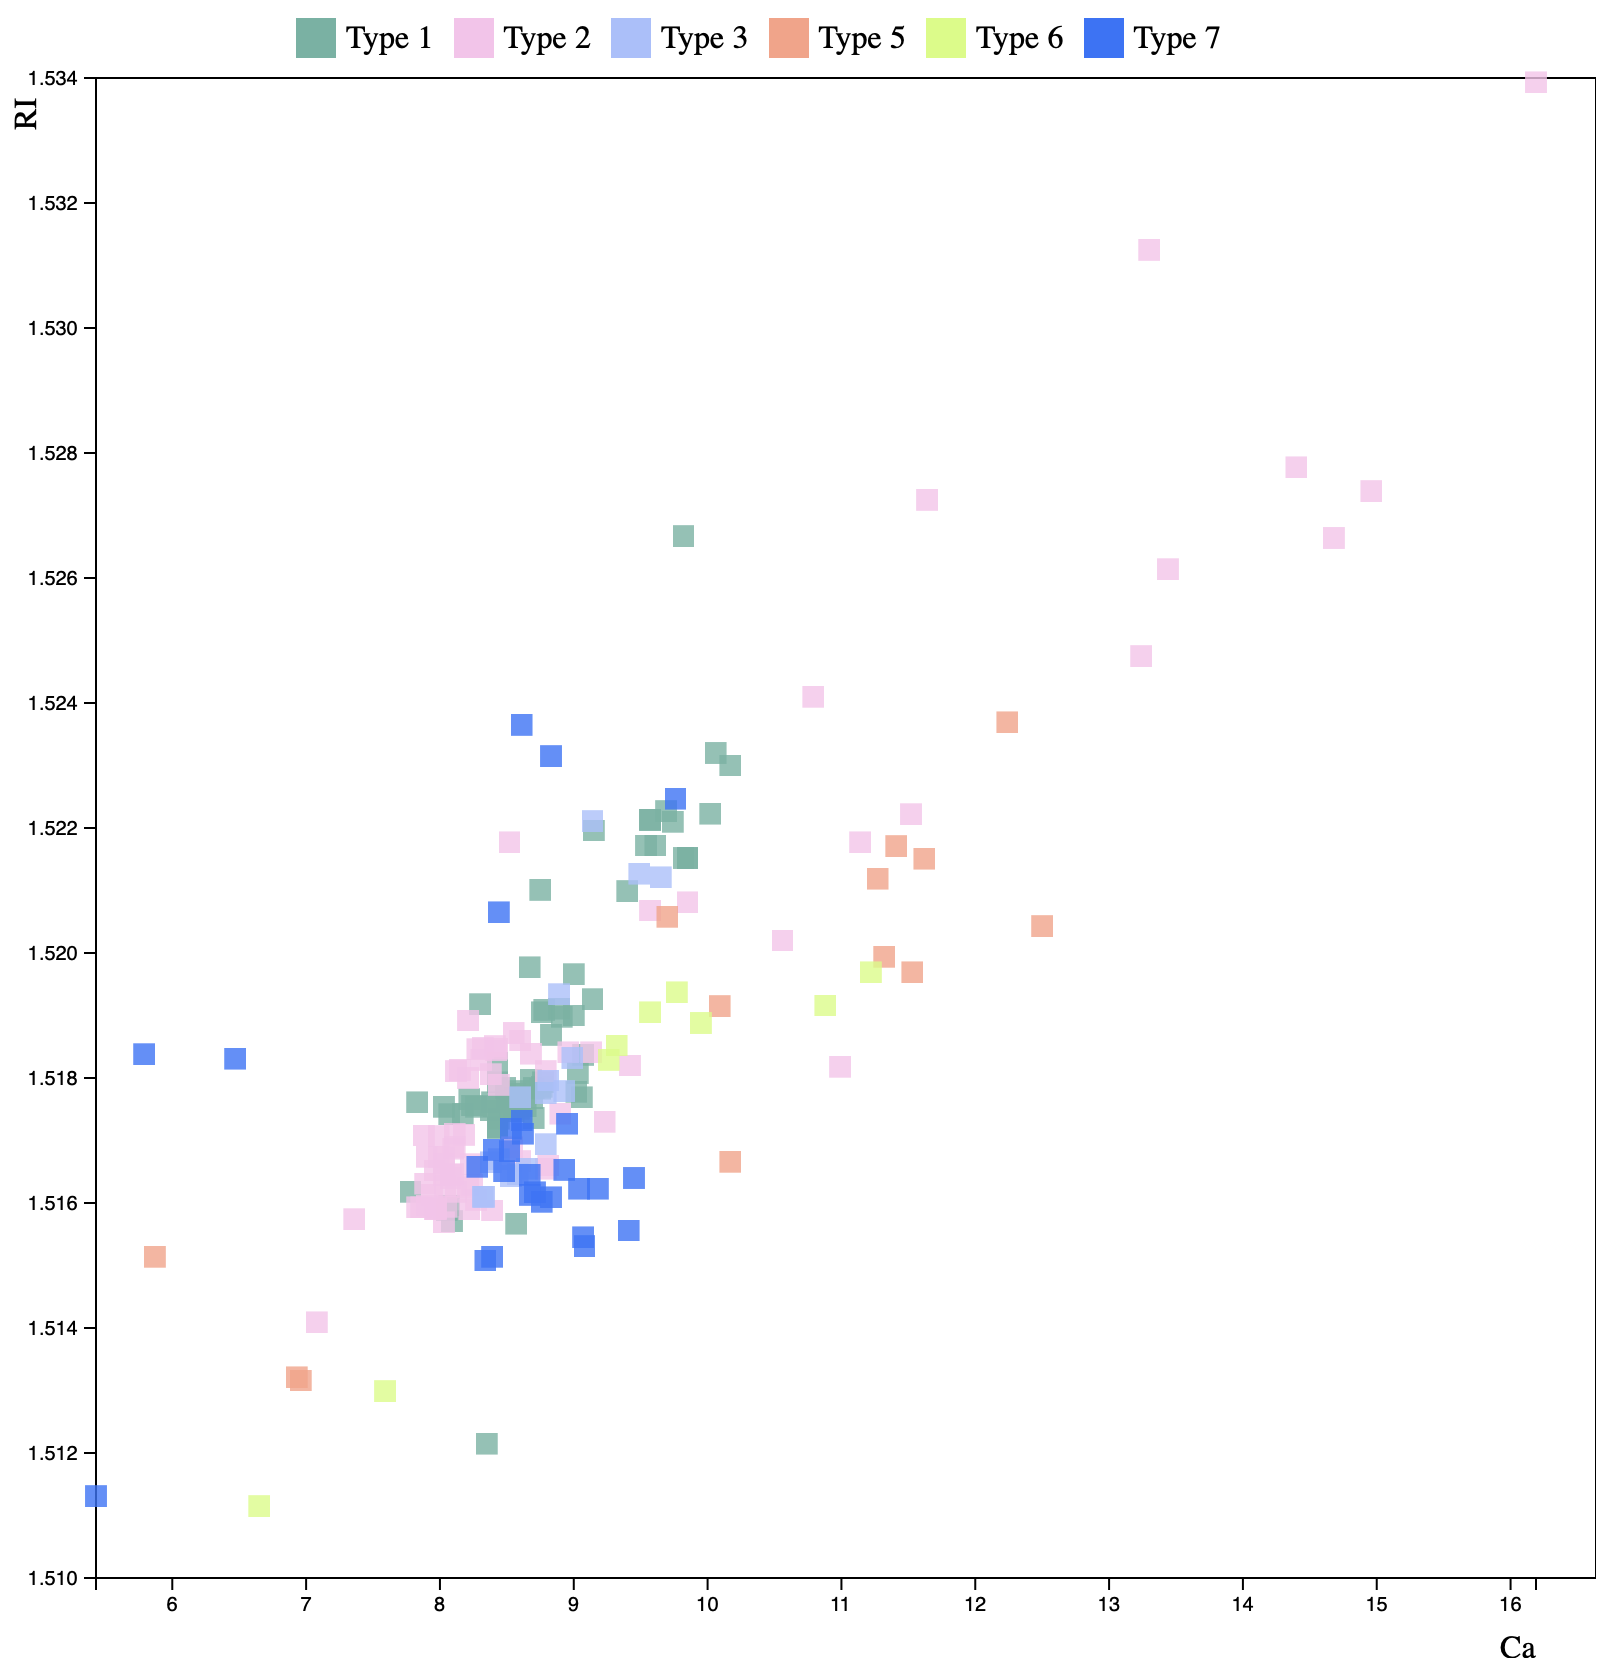
\includegraphics[width=0.55\textwidth]{Task1_2_SP_RI-Ca.png}
\caption{Scatter Plot from columns RI and Ca}
\end{figure}

\newpage

\subsection{Discussion on Visual Analysis 2}

\subsubsection{Design}

\indent

I use R to generate the MDS graph of "glass.csv", and I add the legend for each color to recognize the glass type. After that, I select four types of "two columns" to create graph, and post one of them, the scatterplot from "RI-Ca" as visual analysis 2 scatter plot. The scatter plots are generated through D3.js.

\subsubsection{Evaluation}

\textbf{MDS Graph}

When we evaluate an MDS graph, the main point is to analyze the cluster and outliers.

First, for cluster. It has 2 clusters. One is for Type 7 with yellow points. Another is for Type 1 and 3. The clusters show that the data points related to them are closer in both L1 and L2 distance, and they may have more similar attributes than the others.

Second, for correlation. The Glass Type 7 and Type 2 have some points on the graph that are linear. These points may have only one change in some features. Also some of Type 2 points are not in their line graph. So,  the line for Type 2 points may not be universal. Or, Type 2 may be divided into 2 types.

Third, for outliers. There exist many outliers in the graph for Type 2, 5 and 7. It shows that these points may be errors or special. Considering that the outliers, specifying in these types, the points are likely to be special rather than errors.

\bigskip

\noindent\textbf{Scatter Plot}

From MDS, we know that Glass Type 1, 3 have a cluster, and Type 7 have another. We also find these 2 clusters in the scatter plot. Both 2 graphs tell that the points in clusters have more similarities.

Also, for outliers. we find that Type 2, 5 glass have more outliers in the scatter plot. This also proves what we guess in the MDS graph.

There may be a positive correlation between RI and Ca. But we also know that there exist special points for Type 2. So, the correlation may not be so strong.

\subsubsection{Pros and Cons}

\textbf{MDS Graph}

For advantages. MDS graph can change the multi-dimension data to low-dimension and maintain the data distance. The cluster helps us to find the similarities among multi-dimensional points. The outlier may show errors or special points.

For disadvantages. MDS graph may lose some similarities, as the dimensionality reduction process cannot completely ensure the consistency of distances. In addition, the information on the graph is limited. We must use other graphs, such as scatter plots, to prove similarities or correlations.

\bigskip

\noindent\textbf{Scatter Plot}

The Scatter Plot can easily find the similarities, correlations, and clusters in special 2 dimensions. But it is hard to consider many dimensions at the same time, which may cause information loss when processing multi-dimensional data.

\subsubsection{Comparison}

\indent 

These 2 methods are both processing multi-dimensional data.

When using parallel coordinates, it will be easy to add new dimension data to the visualization. Every dimension and points will be shown in the graph and no information loss. However, it is limited to an analysis of the correlation and similarities. The orders of columns greatly affect the analysis, which increases uncertainty. Also, when handling huge data projects, too many lines intersections bring barriers to the analysis.

When using MDS and scatter plot. It will be easy to find the correlation, cluster and similarities. But these dimension decrease process may cause information loss. The distance between multi-dimensional and low-dimensional may change and cause error in the process. Also, we may need many scatter plots to reach the same effect equal to one parallel coordinates.

\newpage

\section{Category B}

\subsection{Visual Analysis 1}

\begin{figure}[h]
\centering
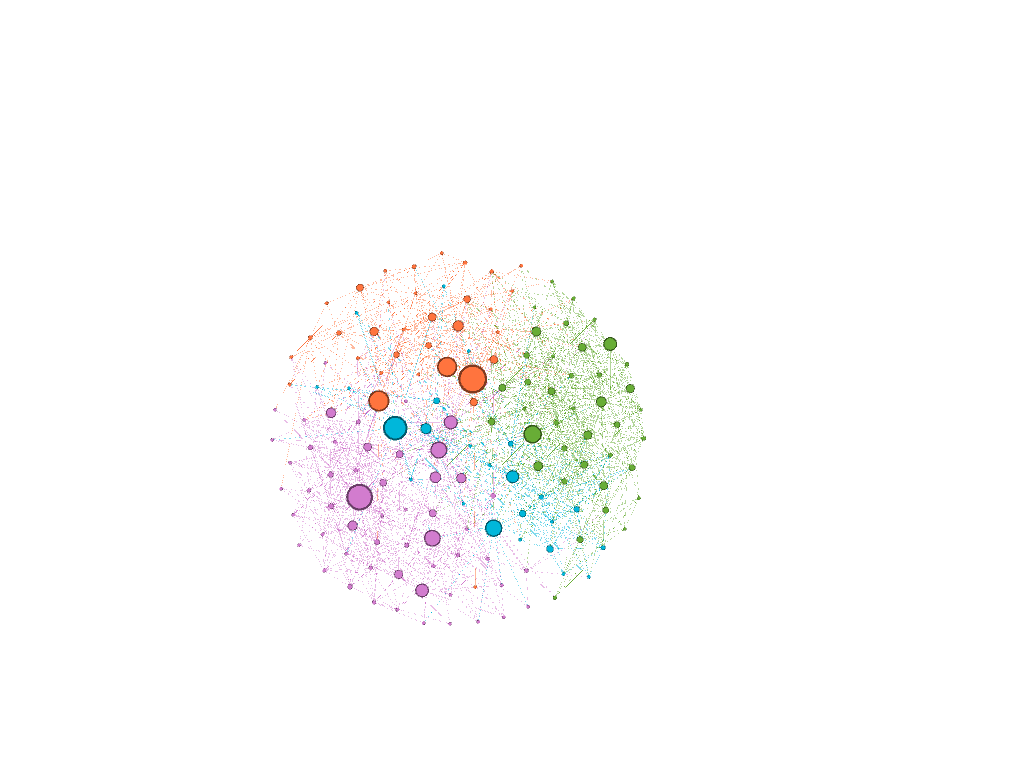
\includegraphics[width=1.2\textwidth]{boardgames-BC-3.png}
\caption{Boardgames Betweenness Centrality Visualiaztion}
\end{figure}

\newpage

\subsection{Discussion on Visual Analysis 1}

\subsubsection{Design}

\noindent

I use networkX to select 150 important points due to their betweenness centrality, then store them in a new gml document. Then I used Gephi to layout this gml graph using the Fruchterman Reingold layout. The point sizes are due to their betweenness centrality, whereas the point color is due to their modularity community detection. 

\subsubsection{Evaluations}

\noindent

According to the thoughts of Betweenness Centrality, a point has greater betweenness centrality if it is on the shortest path between two other points. So when considering the most important points in a network, it may be worked out by comparing the betweenness centrality.

For betweenness centrality. The betweenness centrality of points is shown by their node size. Some of these points are larger than others, such as the orange, blue, and purple points in this graph. These points are the key of the network. They play an important role as bridges in the network. The loss or destruction of these points can seriously undermine network connectivity and efficiency. And we may concentrate on it to improve the connectivity. In real projects, these games may be the origin of other games or have more similarity with others. And learning the important games may be the basic of other games. The Game providers can choose to provide more network resources in key games.

For modularity. Modularity is used to detect the community structure. The modularity value is 0.444, which is on the scale of 0.3-0.7. This means that the cluster effect is great in this project. The 150 boardgames are divided into 4 communities. Each cluster has more internal links. This may mean that 150 important games can be divided into 4 types, and each of them has more similarities. In real projects, the game providers can bundle games from the same cluster to increase sales.

\subsubsection{Pros and Cons}

\noindent

\textbf{Advantages}

From the graph, it can be easily to find clusters and the most important points. This is due to the use of community detection and betweenness centrality. The most important points help us to find the basic or origin of boardgames. The clusters help us find similar boardgames.

\textbf{Disadvantages}

The betweenness centrality may have some differences, compared to degree centrality, closeness centrality, and eigenvector centrality. The betweenness centrality concentrates more on the numbers of closest paths, while degree centrality believes the numbers of edges, closeness centrality believes the shortest distance to other points. Each of them concentrates special points, this may only differ from views to specify 'important points'.

Modularity has barriers to detect small communities. As small communities may be hidden by large communities, it will be hard to research some special communities. In addition, it may need more than normal resources to do modularity in a huge dataset, even through our boardgames.gml being not a huge dataset. 

\newpage

\subsection{Visual Analysis 2}

\begin{figure}[h]
\centering
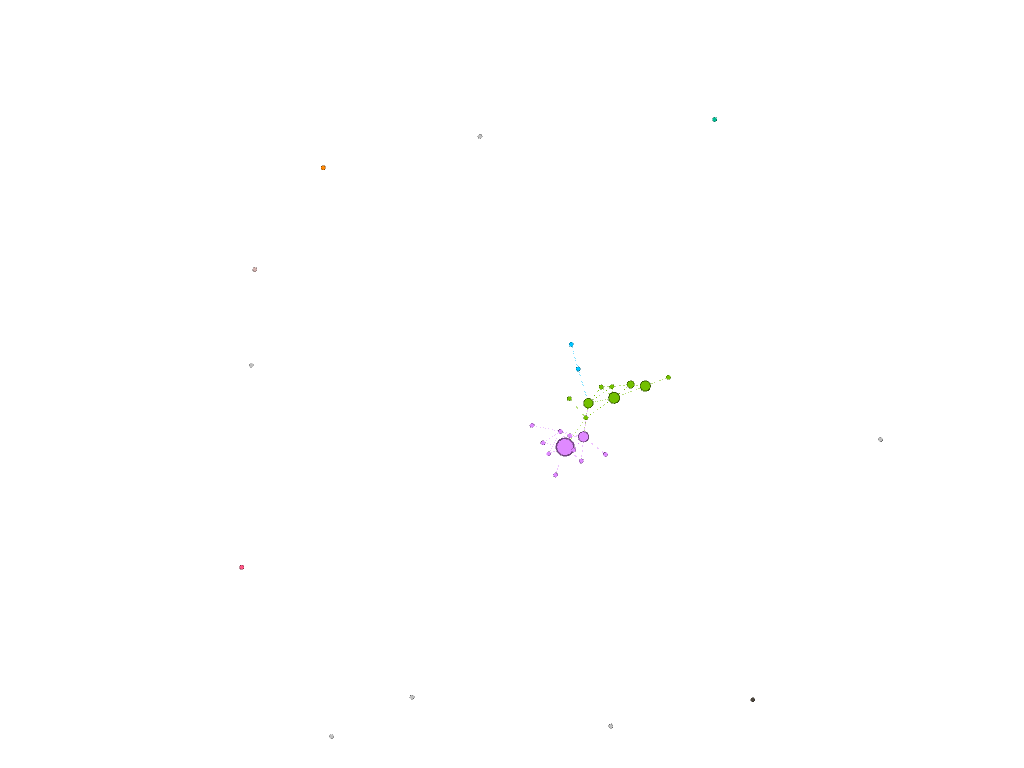
\includegraphics[width=0.65\textwidth]{Animals.png}
\caption{'Animals' Boardgames Visualization}
\end{figure}

\begin{figure}[h]
\centering
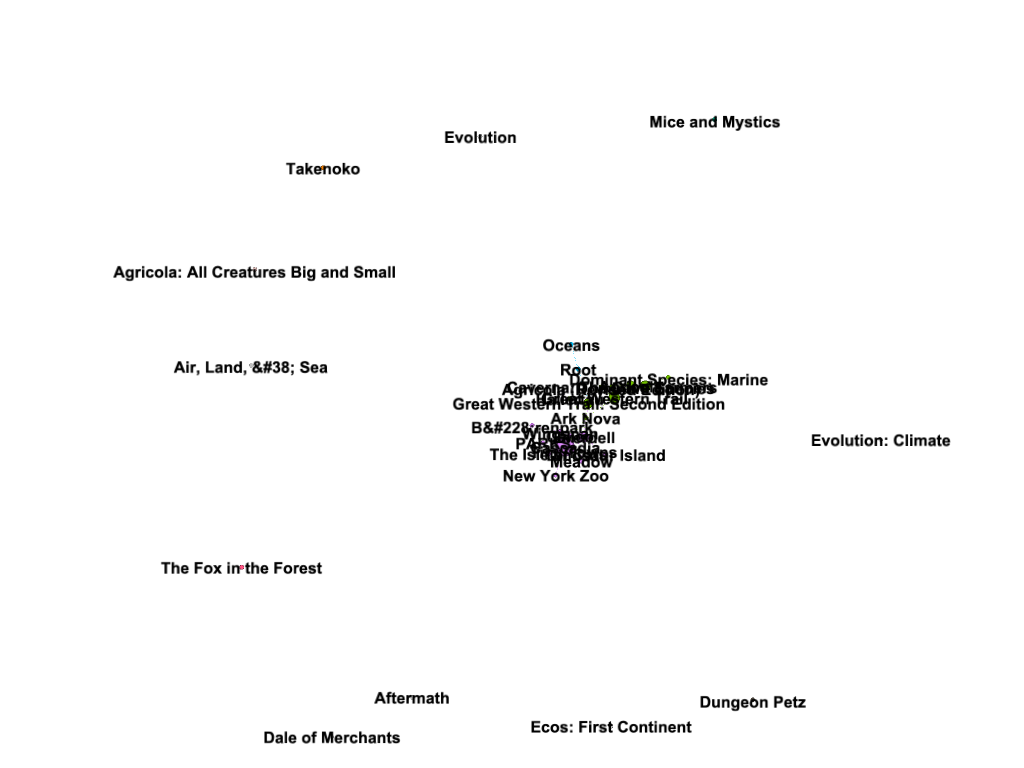
\includegraphics[width=0.65\textwidth]{Animals_labels.png}
\caption{'Animals' Boardgames Visualization with labels}
\end{figure}

\newpage

\begin{figure}[h]
\centering
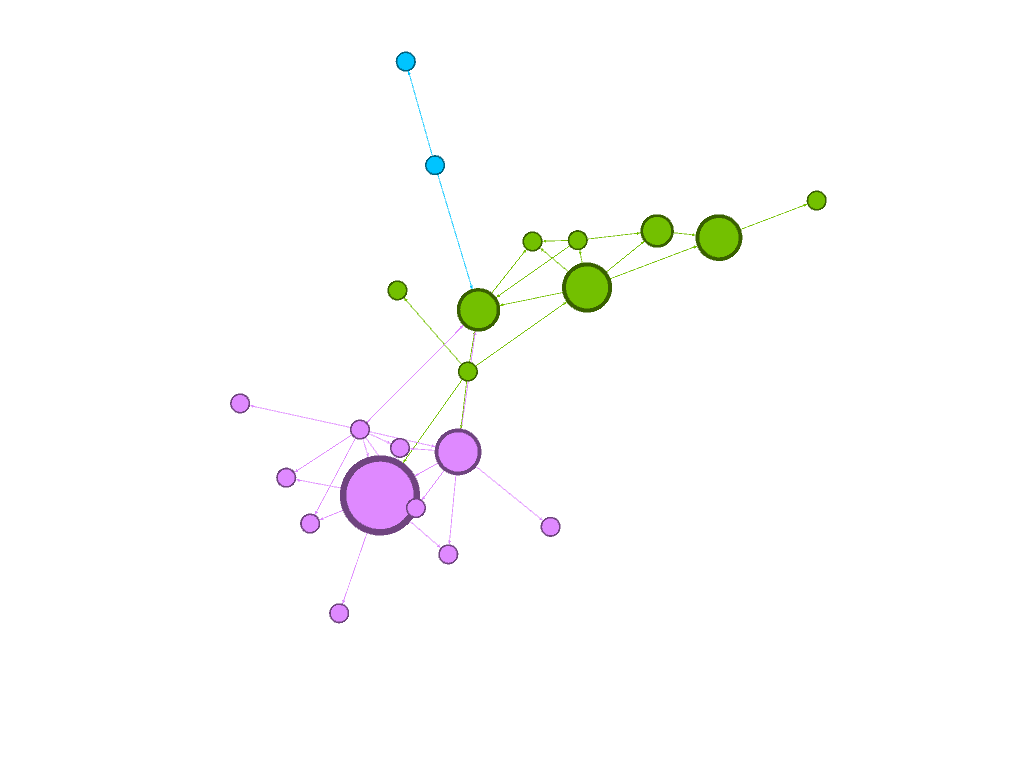
\includegraphics[width=0.7\textwidth]{Animals_central.png}
\caption{The central part of 'Animals' Boardgames Visualization}
\end{figure}

\newpage

\subsection{Discussion on Visual Analysis 2}

\subsubsection{Design}

\noindent

I used NetworkX to select boardgames that have 'Animals' in their 'categories'. There exist 43 games. Then I removed other nodes and generated the gml document for these 43 games. I used Gephi to investigate their betweenness centrality and modularity and to generate the graphs. I used the Yifan Hu layout to show the graph. I used node size to show their betweenness centrality and used node color to show their modularity.

\subsubsection{Evaluations}

\noindent

The evaluation process is similar to Visualization 1.

For betweenness centrality. The central nodes are larger than the edge nodes. This means that some of the central nodes have a higher betweenness centrality. The central node has lines with each other, while the edge one does not. This means that the central nodes games have similarity in 'Animals' contents, while the edge one is only isolated in the 'Animals' element, or the 'Animals' element is not the main one in the edge game.

For modularity. The central nodes are divided into 3 clusters. This means these games can be divided into 3 communities and each community has more similarity. These 3 clusters or communities also have connection with other clusters. But for edge nodes, they have no clusters and are more like several outliers.

For outliers. The graph directly shows their existence. They only have an 'Animals' element, but have no connection with other 'Animals' games. The one reason for this is that they are independently produced games about 'Animals'. Another possible reason is that they may concentrate on other elements, 'Animals' is not the main one.

\subsubsection{Pros and Cons}

\textbf{Advantages}

This graph directly shows clusters and outliers of the 'Animals' nodes. This helps us truly find which games have value to research on its 'Animals' element, and remove outliers from research scale. The modularity and betweenness centrality help us to make sure the research orders (due to its importance) and research comparison (due to its cluster). We may guess the possible reason for this and then prove our prediction in the next lab.

\textbf{Disadvantages}

Like what we do in visualization 1. These visual graphs only concentrate its betweenness centrality, may have ignored in other contrality. The outliers are not deleted, so the central nodes are too small in the graph. The distance between the central node and the edge node is too large.

\subsubsection{Comparison}

\noindent

These two visualization tasks are oriented to different purposes. 

The first task is to find the most important boardgames in 600 games. The importance detection helps us to improve the network connectivity and efficiency. Our research point is to concentrate on which boardgame is the basic or origin one. The nodes in the graph have no outliers. According to the 'importance', no nodes have too few edges.

The second task is to find the relation among the games that have the 'Animals' element. The graphs show clusters and outliers of 'Animals' games. The scope of the research is smaller and more specialized. This will be a benefit in the research on special questions.

\newpage

\appendix

\section{Category A}

\subsection{Visualization 1 Codes}

Parallel coordinates using D3.js.\cite{legend}

\begin{lstlisting}
<!DOCTYPE html>
<meta charset="utf-8">

<head>
    <style>
      #legend {
        display: flex;
        margin-top: 20px;
        margin-left: 150px;
      }
      .legend-item {
        display: flex;
        align-items: center;
        margin-right: 10px;
      }
      .legend-color {
        width: 20px;
        height: 20px;
        margin-right: 5px;
      }
    </style>
  </head>

<body>
<div id="legend"></div>

<!-- load the d3.js library -->    	
<script src="//d3js.org/d3.v7.min.js"></script>
<script>
// set the dimensions and margins of the diagram
var margin = {top: 20, right: 20, bottom: 20, left: 0},
  width = 900 - margin.left - margin.right,
  height = 300 - margin.top - margin.bottom;
var paths;
d3.csv("glass.csv")
    .then(function(data){
        
        // append the svg object to the body of the page
        // appends a 'group' element to 'svg'
        // moves the 'group' element to the top left margin
        var svg = d3.select("body").append("svg")
            .attr("width", width + margin.left + margin.right-100)
            .attr("height", height + margin.top + margin.bottom)
        .append("g")
            .attr("transform",
                    "translate(" + margin.left + "," + margin.top + ")");
        
        
        // Extract the list of dimensions we want to keep in the plot. Here I keep all except the column called Species
        dimensions = Object.keys(data[0]).filter(function(d) { return d != "Type" })

        // Dimensions columns exchange
        function column_exchange(i,j) {
            middle = dimensions[i]
            dimensions[i] = dimensions[j]
            dimensions[j] = middle
        }

        column_exchange(0,8)
        column_exchange(1,5)
        column_exchange(3,6)
        column_exchange(6,7)
        column_exchange(5,6)

        // For each dimension, build a linear scale and store all scales in a y object
        var y = {}
        for (i in dimensions) {
            name = dimensions[i]
            y[name] = d3.scaleLinear()
            .domain( d3.extent(data, function(d) { return +d[name]; }) )
            .range([height, 0])
        }

        // Build the X scale -> it find the best position for each Y axis
        x = d3.scalePoint()
            .range([0, width-100])
            .padding(1)
            .domain(dimensions);

        // The path function take a row of the csv as input, and return x and y coordinates of the line to draw for this raw.
        function path(d) {
            return d3.line()(dimensions.map(function(p) { return [x(p), y[p](d[p])]; }));
        }

        // Color_select scale: input a Type, it outputs a color
        var Color_select = d3.scaleOrdinal()
            .domain(["1", "2", "3", "5", "6", "7"])
            .range([ "#69b3a2", "#fbc2eb", "#a6c0fe", "#fda085", "#d4fc79", "#2575fc"])

        // Draw the lines
        paths = svg
        .selectAll(".myPath")
        .data(data)
        .enter().append("path")
            .attr("d",  path)
            .attr("class", "myPath")
            .style("fill", "none")
            .style("stroke", (function(d) {  return Color_select(d.Type) }))
            .style("opacity", 1)

        // Draw the axis:
        var axes = svg.selectAll(".myAxis")
        // For each dimension of the dataset I add a 'g' element:
        .data(dimensions)
        .enter().append("g")
            // I translate this element to its right position on the x axis
            .attr("transform", function(d) { return "translate(" + x(d) + ")"; })
            .attr("class", "myAxis")
            // And I build the axis with the call function
            .each(function(d) { d3.select(this).call(d3.axisLeft().scale(y[d])); });
        // Add axis title
        axes.append("text")
            .style("text-anchor", "middle")
            .attr("y", -9)
            .text(function(d) { return d; })
            .style("fill", "black");
});

        // Legend Colour
        var legendData = [
        { name: "Type 1", color: "#69b3a2" },
        { name: "Type 2", color: "#fbc2eb" },
        { name: "Type 3", color: "#a6c0fe" },
        { name: "Type 5", color: "#fda085" },
        { name: "Type 6", color: "#d4fc79" },
        { name: "Type 7", color: "#2575fc" }
        ];
        
        // Legend Container
        var legendContainer = d3.select("#legend");
        
        // Legend
        var legendItems = legendContainer.selectAll(".legend-item")
        .data(legendData)
        .enter()
        .append("div")
        .attr("class", "legend-item");
        
        legendItems.append("div")
        .style("background-color", function(d) { return d.color; })
        .attr("class", "legend-color");
        
        legendItems.append("div")
        .text(function(d) { return d.name; })
        .attr("class", "legend-text");

</script>
</body>

\end{lstlisting}

Parallel coordinates using R.

\begin{lstlisting}

# Libraries
library(plotly)


df <- glass

range_min = vector("double", ncol(df))
range_max = vector("double", ncol(df))
labels = vector("character", ncol(df))

for (i in seq_along(df)) {
  range_min[[i]] = min(df[[i]])
  range_max[[i]] = max(df[[i]])
  labels[[i]] = colnames(df)[i]
  
}

fig <- df %>% plot_ly(type = 'parcoords', labelangle=30,
                      

          line = list(color = ~Type,

                      colorscale = 'Viridis'),

          dimensions = list(

            list(range = c(range_min[1],range_max[1]),label = labels[1], values = ~RI),
            list(range = c(range_min[2],range_max[2]),label = labels[2], values = ~Na),
            list(range = c(range_min[3],range_max[3]),label = labels[3], values = ~Mg),
            list(range = c(range_min[4],range_max[4]),label = labels[4], values = ~Al),
            list(range = c(range_min[5],range_max[5]),label = labels[5], values = ~Si),
            list(range = c(range_min[6],range_max[6]),label = labels[6], values = ~K),
            list(range = c(range_min[7],range_max[7]),label = labels[7], values = ~Ca),
            list(range = c(range_min[8],range_max[8]),label = labels[8], values = ~Ba),
            list(range = c(range_min[9],range_max[9]),label = labels[9], values = ~Fe)

            )

          )


fig

\end{lstlisting}

\subsection{Visualization 2 Codes}

MDS using R.

\begin{lstlisting}

glass = read.csv("glass.csv")
glass_dist <- dist(glass[c(1:9)])
glass_mds <- cmdscale((glass_dist))

plot(glass_mds, col = glass$Type, xlab = "MDS L1 Distance", ylab = "MDS L2 Distance", main = "MDS of Glass Types")

legend('topright',
       c("Type 1","Type 2","Type 3","Type 5","Type 6","Type 7"), pch=c(1,1,1,1,1,1), col = c("black", "red", "green", "cyan", "purple", "yellow"))

\end{lstlisting}

Scatter plot using D3.js.\cite{legend}

\begin{lstlisting}

<!DOCTYPE html>
<meta charset="utf-8">

<!-- Load d3.js -->
<script src="https://d3js.org/d3.v7.min.js"></script>

<head>
  <style>
    #legend {
      display: flex;
      margin-top: 20px;
      margin-left: 150px;
    }
    .legend-item {
      display: flex;
      align-items: center;
      margin-right: 10px;
    }
    .legend-color {
      width: 20px;
      height: 20px;
      margin-right: 5px;
    }
  </style>
</head>

<!-- Create a div where the graph will take place -->
<div id="legend"></div>
<div id="glass"></div>
<script>

// set the dimensions and margins of the graph
var margin = {top: 10, right: 30, bottom: 40, left: 50},
    width = 800 - margin.left - margin.right,
    height = 800 - margin.top - margin.bottom;

// append the SVG object to the body of the page
var svg = d3.select("#glass")
  .append("svg")
    .attr("width", width + margin.left + margin.right)
    .attr("height", height + margin.top + margin.bottom)
  .append("g")
    .attr("transform",
          "translate(" + margin.left + "," + margin.top + ")")

// Add the black box around the chart
svg
  .append("rect")
    .attr("x",0)
    .attr("y",0)
    .attr("height", height)
    .attr("width", height)
    .style("fill", "none")
    .style("stroke", "black")

//Read the data
d3.csv("glass.csv").then(function(data) {

  // Add X axis
  var x = d3.scaleLinear()
    .domain(d3.extent(data, function(d) { return +d["Ca"]; }))
    .range([ 0, width ])
  svg.append("g")
    .attr("transform", "translate(0," + height + ")")
    .call(d3.axisBottom(x))

  // Add Y axis
  var y = d3.scaleLinear()
    .domain(d3.extent(data, function(d) { return +d["RI"]; }))
    .range([ height, 0])
    .nice()
  svg.append("g")
    .call(d3.axisLeft(y))

  // Add X axis label:
  svg.append("text")
      .attr("text-anchor", "end")
      .attr("x", width)
      .attr("y", height + margin.top+30)
      .text("Ca");

  // Y axis label:
  svg.append("text")
      .attr("text-anchor", "end")
      .attr("transform", "rotate(-90)")
      .attr("y", -margin.left+20)
      .attr("x", -margin.top)
      .text("RI")

  // Color select: input a Type, it outputs a color
  var Color_select = d3.scaleOrdinal()
      .domain(["1", "2", "3", "5", "6", "7"])
      .range([ "#69b3a2", "#fbc2eb", "#a6c0fe", "#fda085", "#d4fc79", "#2575fc"])

  // Add dots
  svg.append('g')
    .selectAll("dot")
    .data(data)
    .enter()
    .append("path")
      .attr("d", d3.symbol()
        .size(120)
        .type(d3.symbolSquare)
      )
      .attr("transform", function(d) { return "translate(" + x(+d["Ca"]) + "," + y(+d["RI"]) + ")"; })
      .style("fill", (function(d) {  return Color_select(d.Type) }))
      .style("opacity", 0.8)


        // For each Type, input a color to scale it.
        var legendData = [
        { name: "Type 1", color: "#69b3a2" },
        { name: "Type 2", color: "#fbc2eb" },
        { name: "Type 3", color: "#a6c0fe" },
        { name: "Type 5", color: "#fda085" },
        { name: "Type 6", color: "#d4fc79" },
        { name: "Type 7", color: "#2575fc" }
        ];
        
        // Container
        var legendContainer = d3.select("#legend");
        
        // Give out the legend.
        var legendItems = legendContainer.selectAll(".legend-item")
        .data(legendData)
        .enter()
        .append("div")
        .attr("class", "legend-item");
        
        legendItems.append("div")
        .style("background-color", function(d) { return d.color; })
        .attr("class", "legend-color");
        
        legendItems.append("div")
        .text(function(d) { return d.name; })
        .attr("class", "legend-text");

})

</script>

\end{lstlisting}

\newpage

\section{Category B}

\subsection{Visualization 1 Codes}

Selecting 150 the most important nodes through betweenness centrality using NetworkX.

\begin{lstlisting}

import networkx as nx
import matplotlib.pyplot as plt
G = nx.read_gml('boardgames-1.gml')
bc_G = G
bc = nx.betweenness_centrality(bc_G) # BC Process
bc_sort = sorted(bc.items(), key=lambda x:x[1], reverse = True) # Sort
bc_remove = bc_sort[150:] # Select 150 most importment
bc_remove_name = [x[0] for x in bc_remove]

for i in bc_remove_name:
    bc_G.remove_node(i)

nx.draw_spring(bc_G, with_labels = False)

nx.write_gml(bc_G, "boardgames_BC.gml")

\end{lstlisting}

\subsection{Visualization 2 Codes}

Selecting 'Animals' nodes using NetworkX.

\begin{lstlisting}

import networkx as nx
import matplotlib.pyplot as plt
G = nx.read_gml('boardgames-1.gml')
G_remove_label = list()
for i in G.nodes:
    if 'Animals' not in G.nodes[i]['categories']:
        G_remove_label.append(i)

for i in G_remove_label:
    G.remove_node(i)
    
nx.write_gml(G, "boardgames_Animals.gml")

\end{lstlisting}

\bibliographystyle{alpha}
\bibliography{Reference}

\end{document}